\title{GPG in Linux}
\author{Chari Karipidis\\
		2TinG\\}
\date{\today}

\documentclass[12pt]{article}

\usepackage[dutch]{babel}
\usepackage{fancyvrb}
\usepackage{makeidx}
\makeindex
\usepackage{url}
\usepackage{cite}
\usepackage[section]{placeins}
\usepackage{graphicx}
\usepackage{fancyhdr}
\pagestyle{fancy}
\lhead{Chari \textsc{Karipidis}}
\chead{}
\rhead{2TinG}
\lfoot{}
\cfoot{\thepage}
\rfoot{Chari \textsc{Karipidis}}
\renewcommand{\headrulewidth}{0.4pt}
\renewcommand{\footrulewidth}{0.4pt}
\newcommand{\HRule}{\rule{\linewidth}{0.2mm}}
\bibliographystyle{plain}


\begin{document}
	\begin{titlepage}
		\begin{center}
			\textsc{\LARGE Provinciale Hogeschool Limburg}\\[1.5cm]
			\textsc{\large Linux}\\[0.5cm]
			\HRule \\[0.4cm]
			{\huge \bfseries GPG in Linux}\\[0.4cm]
			\HRule \\[1.5cm]
			
			\begin{minipage}{0.4\textwidth}
			\begin{flushleft} \large
			\emph{Author:}\\
			Chari \textsc{Karipidis} 
			\end{flushleft}
			\end{minipage}
			\begin{minipage}{0.4\textwidth}
			\begin{flushright} \large
			\emph{Reviewer:}\\
			Chari \textsc{Karipidis} 
			\end{flushright}
			\end{minipage}
			\vfill
			{\large \today}
		\end{center}
	\end{titlepage}

	\newpage
	\tableofcontents
	
	\newpage
		\section{Introductie}
			In dit document wordt het gebruik van GPG(GnuPG) nader verklaard.

		\paragraph{Benadering}
			De geschiedenis wordt in sectie ~\ref{Geschiedenis} benaderd.
			GPG wordt uitgelegd in Sectie ~\ref{Wat}.
			Hierin wordt de werking en uitvoer via command-line benaderd in secties ~\ref{CLI} en ~\ref{Werk}.
			Ook zijn er Grafische applicaties die met GPG werken. Deze worden benaderd in secties ~\ref{GUI} en ~\ref{Frontend}.
			In de bijlagen sectie ~\ref{Bijlagen} wordt uitgelegd hoe een versiebeheersysteem ingesteld(~\ref{Git}), een mailserver(~\ref{Mail}) 
			en een script voor een mail te verzenden (~\ref{Script}) geconfigureerd worden.
			

		\newpage
		\section{GPG}\label{GPG}
			\subsection{Geschiedenis}\label{Geschiedenis}
				Er is altijd wel een probleem met boodschappen verzenden en ontvangen, zonder dat men deze kan onderscheppen en lezen. Hier zijn handige uitvindingen voor ontworpen, 								die helpen bij dit probleem.

			\paragraph{Scytale}
				In de tijd van de romeinen had men een manier nodig om berichten te versturen naar geallieerde troepen. Verzender en ontvanger waren in het bezit van een 												\textquotedblleft Scytale\textquotedblright\index{Scytale} van ieder dezelfde grootte. Dit voorwerp was een soort van cilinder. Hier werd een riem over gewikkeld en een boodschap 						opgeschreven.\\
				Bij het verwijderen van de riem was deze tekst onleesbaar zonder behulp van de Scytale. De letters waren namelijk door elkaar. Bij ontvangst van de riem bij de 										troepen wikkelden ze de riem over de Scytale die zij bezitten en was het zo mogelijk om de boodschap te lezen.\\
				Dit was een soort van encryptie. Ervoor zorgen dat een onderschepper, de boodschap niet kan lezen.
			\paragraph{Caesar methode}
				Een andere encryptiemethode was de Caesar methode.\\
				Deze bestond uit een zin hervormen m.b.v. het alfabet.\\ 
				Dit klinkt natuurlijk zeer logisch.
				Het alfabet wordt namelijk gebruikt om zinnen te schrijven.\\
				Maar na het schrijven van de nodige boodschap, wordt er een \textquotedblleft sleutel\textquotedblright gekozen. Deze sleutel is een afgesproken cijfer tussen 1 en 26, tussen beide 					partijen.\\
				Belangrijk is dat de cijfers overeenkomen met een letter uit het alfabet. Als het gekozen cijfer 6 is, wordt het alfabet 6 maal naar links verschoven. A wordt dan F 									en B wordt dan G, etc..\\
				De ontvanger krijgt dan een wirwar van letters en kan deze ontcijferen door het alfabet terug te vormen door het 6 maal naar rechts te verschuiven.\\

			\newpage
			\paragraph{Heden}
				Tegenwoordig worden loopjongens niet meer gebruikt. Men is mee ge\"evolueerd naar de toekomst.\\
				Technologie is nu de heerser over het verzenden van boodschappen.
				Mailen, accounts aanmaken, bestanden opslaan, etc.. Gebeurt iedere dag. Dit moet dan ook beveiligd worden.\\
				Dit doen we aan de hand van het encrypteren\index{Encrypteren} van de bestanden, handtekenen van mails,
				etc..
				Een manier voor encryptie is GPG.

			\newpage
			\subsection{Wat is GPG?}\label{Wat}
				GPG of GnuPG staat voor: Gnu Privacy Guard. Zoals de naam al voorstelt, is het om de privacy van gebruikers te beschermen. Dit doormiddel van encryptie van boodschappen 								die verzonden moeten worden zoals mails, data encrypteren, \textquotedblleft sleutelhangers\textquotedblright, etc.. \\
				GnuPG is een commando voor de terminal, zoals te zien in Subsectie~\ref{CLI}, maar er zijn dergelijke frontend\index{Frontend} programma's om deze in een grafische applicatie te 						kunnen gebruiken. Te zien in Subsectie~\ref{GUI}

			\subsection{GPG in command-line interface (CLI)}\label{CLI}
				Zoals ieder ander commando, heeft GPG ook zijn nodige syntax\index{Syntax}.\\
				\begin{center}
					$gpg  [--homedir name]  [--options file]  [options]  command  [args]$\\
				\end{center}
				Het commando \textquotedblleft GPG\textquotedblright heeft een enorm aantal opties. In \textquotedblleft man gpg\textquotedblright worden de opties weergegeven met de nodige uitleg.\\
				In subsecties ~\ref{com}, ~\ref{opt} en ~\ref{use} worden voorbeelden weergegeven van welke er het meest gebruikt worden.\\
				
				\newpage
				\subsubsection{Voorbeelden van vaak gebruikte commando's}\label{com}
					\begin{table}[!ht] \cite{Commando}
						\begin{tabular}{l|l}
								-c				&	Symmetrische encryptie, vraagt voor passphrase\index{Passphrase}.\\
								--decrypt			&	Decryptie\index{Decryptie} van ge\"encrypteerde bestanden.\\
								--encrypt			&	Encryptie van data. Wordt gecombineerd met -sign.\\
								-sign				&	Maakt handtekening, wordt gecombineerd met --encrypt.\\
								--encrypt-files	&	Encryptie van meerdere bestanden in 1 commando.\\
								--decrypt-files	&	Decryptie van meerdere bestanden in 1 commando.\\
						\end{tabular}
						\caption{Vaak gebruikte commando's}						
					
				\subsubsection{Voorbeelden van vaak gebruikte opties}\label{opt}\cite{Commando}					
						\begin{tabular}{l|l}
								-o file				&	Schrijft output naar \textquotedblleft file\textquotedblright.\\
								--default-key name	&	Standaard waarde voor ID encryptie.\\
								-r name				&	Encryptie naar ontvanger \textquotedblleft name\textquotedblright.\\
								-v					&	Verbose\index{Verbose}, geeft meer info tijdens het proces.\\
								-i					&	Interactief, geeft prompts\index{Prompts} voor iedere stap.\\
						\end{tabular}\caption{Vaak gebruikte opties}
											
				\subsubsection{Voorbeelden van het gebruik}\label{use}\cite{Commando}
						\begin{tabular}{l|l}
								$gpg -r Bob file$				&	Handteken en encryptie voor Bob.\\
								$gpg --clearsign file$			&	Maakt een lege handtekening\index{Handtekening}.\\
								$gpg --fingerprint user_ID$		&	Laat vingerafdruk zien.\\
								$gpg --verify gpgfile$			&	Verifieert pgpfile.\\
								$gpg --list-keys user_ID$		&	Laat sleutels zien.\\
						\end{tabular}
						\caption{Voorbeelden}
					\end{table}	
				\cite{Tabellen}
			
			\newpage		
			\subsection{Werking en uitvoer van GPG}\label{Werk}	
				\paragraph*{Sleutel} 
				Om een bestand te kunnen encrypteren, is een sleutel vereist.\\
				Deze moet als initieele stap worden aangemaakt met het commando:\\
				gpg --gen-key\\
				Bij het gebruik van dit commando worden veel vragen gesteld ter configuratie.\\
				-type van sleutel, -grootte, -vervaldatum, -identificatie.\\
				Na het ingeven van deze waardes wordt er gevraagd naar een Passphrase.
				Deze is zeer belangrijk te onthouden.\\
				Door het commando:\\
				\textquotedblleft  gpg --armor --output pubkey.txt --export 'Naam' \textquotedblright\\
				te gebruiken, zal een uitvoer gemaakt worden van deze public key naar textbestand,
				om deze te kunnen verzenden naar de gewenste contacten.\\
				Zie figuur ~\ref{Terminal}\\
				
				\begin{figure}
					\begin{center}
						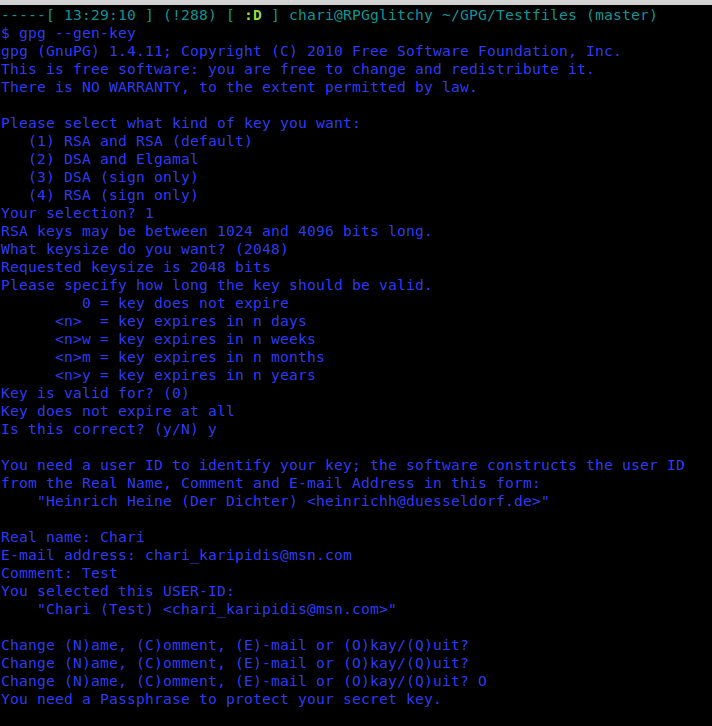
\includegraphics[scale=0.4]{Pictures/Sleutel1}
						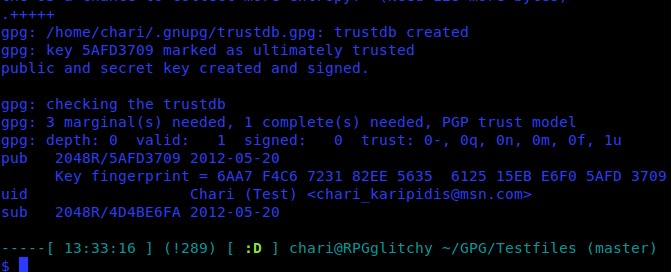
\includegraphics[scale=0.4]{Pictures/Sleutel2}
						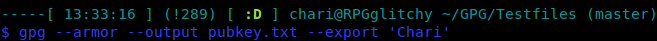
\includegraphics[scale=0.4]{Pictures/Sleutel3}
					\end{center}
					\caption{Sleutel}\label{Terminal}
				\end{figure}
				
				\paragraph{Encryptie en decryptie} \cite{GPGstart}
				gpg --encrypt --recipient \textquotedblleft Naam\textquotedblright test.txt\\
				Door dit commando te gebruiken, zal het bestand \textquotedblleft test.txt\textquotedblright ge\"encrypteerd worden
				met de sleutel van *Naam*.\\
				Na het gebruik van dit commando, werd het bestand \textquotedblleft test.txt\textquotedblright ge\"encrypteerd naar
				\textquotedblleft test.txt.gpg\textquotedblright.
				Als er gewenst wordt, dit bestand te decrypteren, dan gebruiken we het volgende 
				commando:\\
				gpg --output test.txt --decrypt test.txt.gpg\\
				Zie figuur ~\ref{Encryptie}\\
				
				\begin{figure}[!ht]
					\begin{center}
						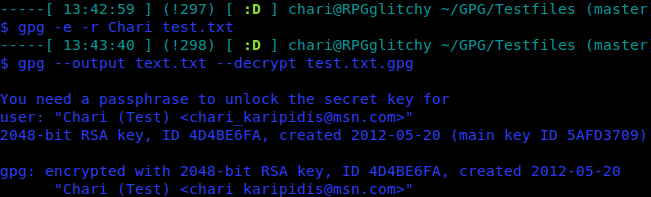
\includegraphics[scale=0.4]{Pictures/Encryptie}
					\end{center}
					\caption{Encryptie}\label{Encryptie}
				\end{figure}
				
				\paragraph{}
				De voorgaande methode is bestemd voor persoonlijk gebruik.\\
				Om te encrypteren naar andere contacten maken we gebruik van het commando 
				\textquotedblleft importeren\textquotedblright: gpg --import key.asc\\
				In dit commando geldt dat \textquotedblleft key\textquotedblright de sleutel is van de persoon die gecontacteerd
				moet worden.\\
				Een andere mogelijkheid is deze sleutel zoeken op een publieke website:\\
				gpg --search-keys \textquotedblleft myfriend@his.isp.com\textquotedblright --keyserver hkp://subkeys.pgp.net\\
				Bij het encrypteren van een bestand, wordt er gebruik gemaakt van dezelfde commando,
				als bij persoonlijk gebruik, maar met een verschillende sleutel.\\
				gpg --encrypt --recipient \textquotedblleft myfriend@his.isp.net\textquotedblright test.txt\\		
				\cite{GPGstart}
			
			\subsection{Frontend GPG programma's}\label{GUI} \cite{Frontend} 
				\begin{table}[!ht]
					\begin{center}
						\begin{tabular}{r|l}
							Cryptophane	&	Een applicatie voor Windows.\\
							Gajim		&	Een Jabber client voor GNOME.\\ \index{Jabber client}
							GnuPG Shell	&	Een cross-platform, grafische Frontend voor GnuPG.\\ \index{Cross-platform}
							GPA			&	De standaard Frontend voor GPG.\\
							KGpg		&	GnuPG voor KDE.\\ \index{KDE}
							Seahorse	&	GnuPG voor GNOME.\\ \index{GNOME}
							Wija		&	Een cross-platform jabber client (MacOsX, Linux, Windows)\\
						\end{tabular}
					\end{center}
					\caption{Gui Frontends} 
				\end{table}
				
			
				\begin{figure}[!ht]
					\paragraph{Cryptophane}
						Deze wordt gebruikt om te encrypteren, decrypteren, handtekenen, beheer van sleutelhanger en een command-line interface voor GnuPG.\\
					\begin{center}
						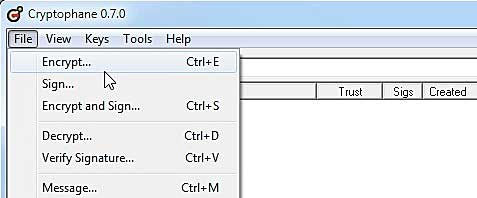
\includegraphics[scale=0.6]{Pictures/cryptophane}
					\end{center}
					\caption{Cryptophane}
				
					\paragraph{Gajim}
						Gajim is een Jabber-client. Een Jabber-client is een messaging applicatie.
						Omdat Gajim werkt met GnuPG, zullen de berichten die verzonden worden met Gajim, ge\"encrypteerd worden.
					\begin{center}
						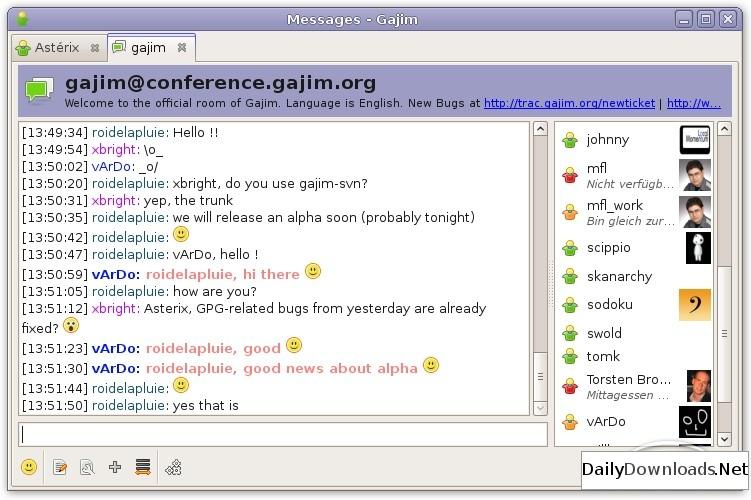
\includegraphics[scale=0.4]{Pictures/gajim}
					\end{center}
					\caption{Gajim}
				\end{figure}
				
				\begin{figure}[!ht]
					\paragraph{GPGshell}\cite{Shell}
						Een grafische frontend voor iedere platform. Met deze GUI \index{GUI} is het mogelijk sleutels bij te houden en te encrypteren. 
					\begin{center}
						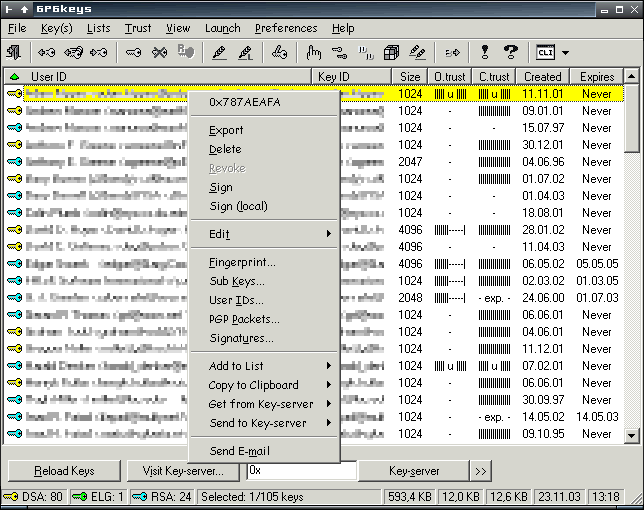
\includegraphics[scale=0.5]{Pictures/gpgshell}
					\end{center}
					\caption{GnuPG Shell}
				
					\paragraph{GPA}
						GPA probeert de standaard frontend te zijn voor GPG. $www.gnupg.org$ Host GPA.
					\begin{center}
						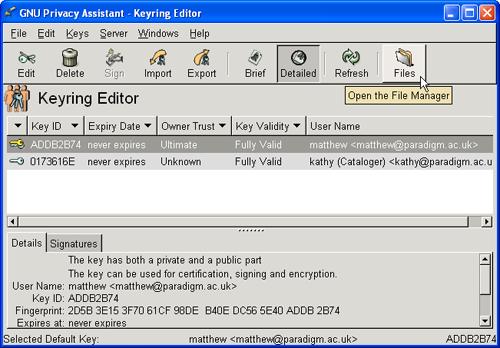
\includegraphics[scale=0.6]{Pictures/GPA}
					\end{center}
					\caption{GPA}
				\end{figure}
				
				\begin{figure}[!ht]				
					\paragraph{KGpg}\cite{Kgpg}
						Met KGpg kan je bestanden en mails encrypteren en decrypteren om je informatie veilig te houden.
						Het is een gratis en open-source\index{Open-source} frontend.
					\begin{center}
						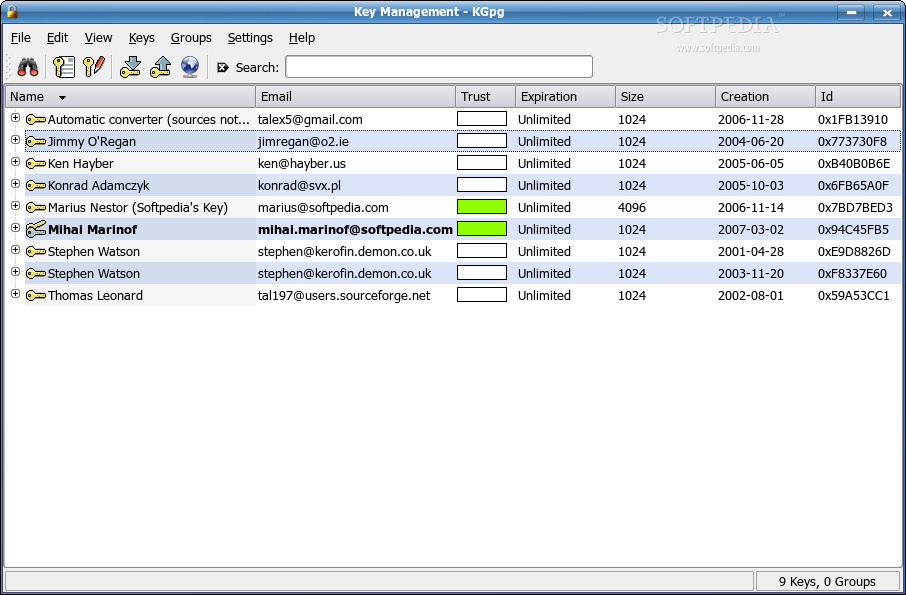
\includegraphics[scale=0.2]{Pictures/kgpg}
					\end{center}
					\caption{KGpg}
				
					\paragraph{Seahorse} \cite{Seahorse}
						Seahorse is een GUI voor GNOME. Het is ook geïntegreerd in Nautilus\index{Nautilus}, gedit en andere applicaties voor encryptie uit te voeren.
						De gebruiker kan met Seahorse PGP en SSH\index{SSH} sleutels maken en beheren, publiceren en terughalen van sleutels op de servers, een passphrase opslaan in het cache 								geheugen, sleutelhanger backuppen, etc..
					\begin{center}
						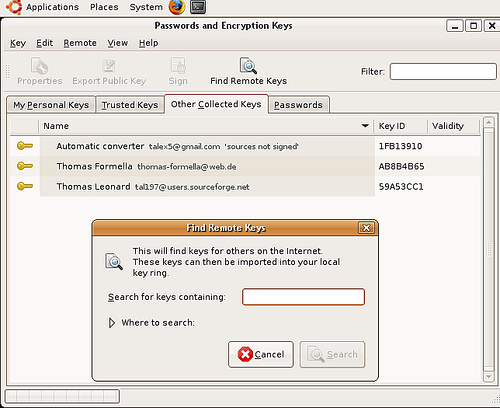
\includegraphics[scale=0.4]{Pictures/Seahorse}
					\end{center}
					\caption{Seahorse}
				\end{figure}
				
				\begin{figure}[!ht]				
					\paragraph{Wija}
						Een Jabber-client zoals Gajim, maar geschreven in java en beschikbaar voor ieder platform.
						Het heeft een ingebouwde sleutelhanger beheersysteem. Het kan ook zeer gemakkelijk boodschappen encrypteren en decrypteren voor gewone gesprekken of 													multi-user gesprekken.
						Het is ook mogelijk de boodschappen te handtekenen.
					\begin{center}
						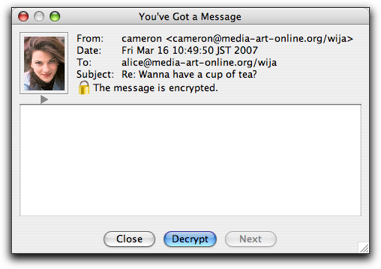
\includegraphics[scale=0.7]{Pictures/wija}
					\end{center}
					\caption{Wija}
				\end{figure}
				
		\subsection{Werking van een GPG Frontend}\label{Frontend}
			Een grafische applicatie voor het gebruik met GPG houdt heel vaak in dat een bestand
			geladen wordt en de gebruiker dan kan kiezen om te encrypteren of decrypteren.\\
			Als de Frontend gebruik maakt van een messaging applicatie (Jabber-client),
			Houdt dit meestal in dat de gebruiker een handtekening instelt in de GUI,
			zodat deze gebruikt wordt bij het encrypteren van de boodschappen.\\
			Als de GUI een sleutelhanger-functie heeft, zal er een instelling van een \textquotedblleft Passphrase\textquotedblright
			Voorzien zijn bij de initieele stappen. Deze passphrase zorgt ervoor dat de sleutelhanger
			ontgrendelt kan worden voor gebruik. Als er dan een wachtwoord wordt ingesteld op een
			website of applicatie, Zal er worden gevraagd deze op te slaan in je sleutelhanger.
			Als de gebruiker dit toestaat, wordt deze ge\"encrypteerd toegevoegd aan je sleutelhanger.
			
		\newpage
		\bibliography{myBib}
		\newpage
		\listoffigures
		\listoftables
		\newpage
		\printindex	
			
		\section{Bijlagen}\label{Bijlagen}
			\subsection{Versiebeheersysteem}\label{Git}
				\subsubsection{Registratie}
					De eerste stap om een versiebeheersysteem te kunnen aanmaken, is het registreren op een website die versiebeheersysteem beheert.\\
					$www.github.com$ Is een beheerder van versiebeheersystemen.\\
					Bij het registreren op Github wordt er nadien een ronde gedaan om te helpen bij het configureren van iemands bewaarplaats.
					
				\subsubsection{Configuratie}
					Via \textquotedblleft Synaptic Package Manager\textquotedblright is het nodig, bepaalde pakketen te downloaden, namelijk: \textquotedblleft git-core\textquotedblright, 								\textquotedblleft git-doc\textquotedblright, \textquotedblleft git-gui\textquotedblright.\\
					Github maakt gebruikt van SSH sleutels voor een veilige connectie.\\
					Met de volgende commando's in de terminal, wordt er een eigen SSH sleutel aangemaakt.\\
					Eerst, bestaande SSH sleutels backuppen en verwijderen.\\
					\\
					mkdir key\_backup\\
					cp id\_rsa* key\_backup\\
					rm id\_rsa*
					\\
					\\
					 Daarna een nieuwe SSH sleutel genereren.\\
					 \\
					 ssh-keygen -t rsa -C \textquotedblleft uw\_email@uwemail.com"\\
					 \\
					 De terminal vraagt de gebruiker voor een passphrase.
					 Na ingave van de passphrase is de SSH sleutel ingesteld.\\
					Deze sleutel moet toegevoegd worden in github. De volgende stappen laten zien hoe dat gebeurd.\\
					 Open id-rsa.pub en kopieer de inhoud van dit bestand.\\
					 In de tab \textquotedblleft Instellingen\textquotedblright op Github, bij \textquotedblleft SSH Keys\textquotedblright is het mogelijk een Sleutel toe te voegen.\\
					 Bij het drukken op \textquotedblleft Add SSH key\textquotedblright kan de gekopieerde tekst toegevoegd worden en opgeslaan.\\
					 \\
					 Het versiebeheersysteem kan met de SSH sleutel nu getest worden door het volgende commando:\\
					 \\
					 ssh -T git@github.com\\
					 \\
					 Hier zal worden gevraagd om verder te gaan en zal dan de gebruiker begroeten en toegang bieden.\\
					 \\
					 De laatste stap bestaat uit configuratie van git.\\
					 git config --global user.name "Voornaam Achternaam"\\
					 git config --global user.email \textquotedblleft uwemail@uwemail.com"\\
					 \\
					 Deze commando's zorgen voor een correcte configuratie van git.\\
					 \\
				\cite{Git}				
				
				\newpage
				\subsubsection{Git commando's}
					Nadat het versiebeheersysteem correct is geconfigureerd, kan er een bewaarplaats worden aangemaakt.\\
					Door op \textquotedblleft New repository\textquotedblright te klikken is het mogelijk een bewaarplaats aan te maken in een bestaand account.\\
					Met behulp van volgende commando's, kunnen bestanden in een bepaald pad worden toegevoegd aan de git.\\
					\\
					 mkdir ~/Hello-World\\
					 cd ~/Hello-World\\
					 git init\\
					 \\
					 Door git init, wordt een connectie ge\"initialiseerd tussen github en het pad.\\
					 Als er nu bestanden worden toegevoegd in deze map, kan er met de volgende commando's, bestanden toegevoegd worden aan git.\\
					 \\
					  git status (laat zien welke bestanden verandert zijn)\\
					  git add *naam (voegt bestand met naam *naam toe)\\
					  git commit -m \textquotedblleft boodschap voor verandering\textquotedblright\\
					  git remote add origin git@github.com:gebruikersnaam/Hello-World.git\\
					  git push -u origin master (eerst een origin master aanmaken voor een beheer op afstand)\\
					  \\
					  Nadat er voor het eerst een origin master wordt aangemaakt en \textquotedblleft pushed\textquotedblright,\\
					  Zal er in de toekomst enkel \textquotedblleft git push\textquotedblright gebruikt kunnen worden.
			
			\newpage
			\subsection{Mailserver configuratie}\label{Mail}
				\subsubsection{Mailserver instellen}
					Om mutt te installeren, wordt er gebruik gemaakt van een simpel commando.\\
					\\					
					sudo apt-get install openssl mutt\\
					\\
					Alle gevraagde waardes mogen standaard zijn.\\
					Mutt is nu succesvol geïnstalleerd.
					
				\subsubsection{Configuratie}
					Ter configuratie moet een bestand \textquotedblleft .muttrc\textquotedblright aangemaakt worden in de homefolder.\\
					Dit bestand moet de volgende inhoud bevatten:\\
						\\
						set imap\_user = \textquotedblleft username@gmail.com"\\
						set imap\_pass = "password"\\
						\\
						set smtp\_url = "smtp://username@smtp.gmail.com:587/"\\
						set smtp\_pass = "password"\\
						set from = \textquotedblleft username@gmail.com"\\
						set realname = "Your Real Name"\\
						\\
						set folder = \textquotedblleft imaps://imap.gmail.com:993"\\
						set spoolfile = "+INBOX"\\
						set postponed="+[Gmail]/Drafts"\\
						\\
						set header\_cache=~/.mutt/cache/headers\\
						set message\_cachedir=~/.mutt/cache/bodies\\
						set certificate\_file=~/.mutt/certificates\\
						\\
						set move = no\\
						\\
					In dit bestand moeten de \textquotedblleft username\textquotedblright, \textquotedblleft password\textquotedblright en \textquotedblleft Your Real Name\textquotedblright 								gepersonaliseerd worden.\\
			\cite{Mail}
					
			\subsection{Bash-script}\label{Script}
				\VerbatimInput[baselinestretch=1,fontsize=\footnotesize,numbers=left]{Mailreviewer.sh} 
				\paragraph{Script}				
				Het script zal respectievelijk de aanspreking, voornaam, naam, e-mailadres en het pad naar de .tex file vragen.\\
				Na ingave wordt er een controle uitgevoerd op de gegevens.\\
				Er wordt een backup gemaakt van het .tex bestand om fouten te vermijden.\\
				Door het \textquotedblleft sed\textquotedblright commando wordt een gegeven stuk tekst vervangen door een ander stuk tekst.\
				In dit geval wordt \textquotedblleft Xname\textquotedblright vervangen door \textquotedblleft naam + voornaam \textquotedblright .\\
				Om dit te laten verschijnen in de pdf, gebruikt het script de \textquotedblleft pdflatex\textquotedblright commando. \\
				Heel de directory van LaTex wordt als volgt Gearchiveerd. Hier wordt een uitvoer geschreven naar een tekstbestand.\\
				De gebruiker krijgt de optie om een bericht toe te voegen aan de mail, voor deze verzonden wordt.\\
				Na het succesvol verzenden, worden de tijdelijke bestanden (Zip en tekstbestanden) verwijdert.\\
				Ten slotte wordt de optie voorgelegd om de backup terug te plaatsen als origineel bestand.\\

\end{document}
